\def\year{2022}\relax
%File: formatting-instructions-latex-2022.tex
%release 2022.1
\documentclass[letterpaper]{article} % DO NOT CHANGE THIS
\usepackage{aaai22}  % DO NOT CHANGE THIS
\usepackage{times}  % DO NOT CHANGE THIS
\usepackage{helvet}  % DO NOT CHANGE THIS
\usepackage{courier}  % DO NOT CHANGE THIS
\usepackage[hyphens]{url}  % DO NOT CHANGE THIS
\usepackage{graphicx} % DO NOT CHANGE THIS
\urlstyle{rm} % DO NOT CHANGE THIS
\def\UrlFont{\rm}  % DO NOT CHANGE THIS
\usepackage{natbib}  % DO NOT CHANGE THIS AND DO NOT ADD ANY OPTIONS TO IT
\usepackage{caption} % DO NOT CHANGE THIS AND DO NOT ADD ANY OPTIONS TO IT
\DeclareCaptionStyle{ruled}{labelfont=normalfont,labelsep=colon,strut=off} % DO NOT CHANGE THIS
\frenchspacing  % DO NOT CHANGE THIS
\setlength{\pdfpagewidth}{8.5in}  % DO NOT CHANGE THIS
\setlength{\pdfpageheight}{11in}  % DO NOT CHANGE THIS
%
% These are recommended to typeset algorithms but not required. See the subsubsection on algorithms. Remove them if you don't have algorithms in your paper.
\usepackage{algorithm}
\usepackage{algorithmic}

%
% These are are recommended to typeset listings but not required. See the subsubsection on listing. Remove this block if you don't have listings in your paper.
\usepackage{newfloat}
\usepackage{listings}
\lstset{%
	basicstyle={\footnotesize\ttfamily},% footnotesize acceptable for monospace
	numbers=left,numberstyle=\footnotesize,xleftmargin=2em,% show line numbers, remove this entire line if you don't want the numbers.
	aboveskip=0pt,belowskip=0pt,%
	showstringspaces=false,tabsize=2,breaklines=true}
\floatstyle{ruled}
\newfloat{listing}{tb}{lst}{}
\floatname{listing}{Listing}
%
%\nocopyright
%
% PDF Info Is REQUIRED.
% For /Title, write your title in Mixed Case.
% Don't use accents or commands. Retain the parentheses.
% For /Author, add all authors within the parentheses,
% separated by commas. No accents, special characters
% or commands are allowed.
% Keep the /TemplateVersion tag as is
\pdfinfo{
/Title (Ludus: An Optimization Framework to Balance Auto Battler Cards)
/Author (Nathaniel Budijono, Phoebe Goldman, Jack Maloney, Joseph B. Mueller, Phillip Walker, Jack Ladwig, Richard G. Freedman)
/TemplateVersion (2022.1)
}
%/Author (Anonymous)
% Alternate name: BaOBAB (Balance Optimizer with Benchmarks in Auto Battlers)

% DISALLOWED PACKAGES
% \usepackage{authblk} -- This package is specifically forbidden
% \usepackage{balance} -- This package is specifically forbidden
% \usepackage{color (if used in text)
% \usepackage{CJK} -- This package is specifically forbidden
% \usepackage{float} -- This package is specifically forbidden
% \usepackage{flushend} -- This package is specifically forbidden
% \usepackage{fontenc} -- This package is specifically forbidden
% \usepackage{fullpage} -- This package is specifically forbidden
% \usepackage{geometry} -- This package is specifically forbidden
% \usepackage{grffile} -- This package is specifically forbidden
% \usepackage{hyperref} -- This package is specifically forbidden
% \usepackage{navigator} -- This package is specifically forbidden
% (or any other package that embeds links such as navigator or hyperref)
% \indentfirst} -- This package is specifically forbidden
% \layout} -- This package is specifically forbidden
% \multicol} -- This package is specifically forbidden
% \nameref} -- This package is specifically forbidden
% \usepackage{savetrees} -- This package is specifically forbidden
% \usepackage{setspace} -- This package is specifically forbidden
% \usepackage{stfloats} -- This package is specifically forbidden
% \usepackage{tabu} -- This package is specifically forbidden
% \usepackage{titlesec} -- This package is specifically forbidden
% \usepackage{tocbibind} -- This package is specifically forbidden
% \usepackage{ulem} -- This package is specifically forbidden
% \usepackage{wrapfig} -- This package is specifically forbidden
% DISALLOWED COMMANDS
% \nocopyright -- Your paper will not be published if you use this command
% \addtolength -- This command may not be used
% \balance -- This command may not be used
% \baselinestretch -- Your paper will not be published if you use this command
% \clearpage -- No page breaks of any kind may be used for the final version of your paper
% \columnsep -- This command may not be used
% \newpage -- No page breaks of any kind may be used for the final version of your paper
% \pagebreak -- No page breaks of any kind may be used for the final version of your paperr
% \pagestyle -- This command may not be used
% \tiny -- This is not an acceptable font size.
% \vspace{- -- No negative value may be used in proximity of a caption, figure, table, section, subsection, subsubsection, or reference
% \vskip{- -- No negative value may be used to alter spacing above or below a caption, figure, table, section, subsection, subsubsection, or reference

\setcounter{secnumdepth}{2} %May be changed to 1 or 2 if section numbers are desired.

% The file aaai22.sty is the style file for AAAI Press
% proceedings, working notes, and technical reports.
%

% Title

% Your title must be in mixed case, not sentence case.
% That means all verbs (including short verbs like be, is, using,and go),
% nouns, adverbs, adjectives should be capitalized, including both words in hyphenated terms, while
% articles, conjunctions, and prepositions are lower case unless they
% directly follow a colon or long dash
%\iffalse
%Example, Multiple Authors, ->> remove \iffalse,\fi and place them surrounding AAAI title to use it
\title{{\sc Ludus}: An Optimization Framework to Balance Auto Battler Cards}
% Framework, No metric exploration, Optimizing (not just balance)
%%Finding the Balance: An Exploration of Metrics to Design Balanced Character Stats in Auto Battler Games
\author {
    %Submission \# 40
%\if{false}
    % Authors
    Nathaniel Budijono\equalcontrib,\textsuperscript{\rm 1}
    Phoebe Goldman\equalcontrib, \textsuperscript{\rm 2}
    Jack Maloney\equalcontrib, \textsuperscript{\rm 3} \\
    Joseph B. Mueller, \textsuperscript{\rm 4,5}
    Phillip Walker, \textsuperscript{\rm 5}
    Jack Ladwig, \textsuperscript{\rm 5}
    Richard G. Freedman \textsuperscript{\rm 5}
%\fi
}
\affiliations {
%\if{false}
    % Affiliations
    \textsuperscript{\rm 1} University of Minnesota Twin Cities\\
    \textsuperscript{\rm 2} New York University\\
    \textsuperscript{\rm 3} University of Wisconsin-Madison\\
    \textsuperscript{\rm 4} University of Minnesota\\
    \textsuperscript{\rm 5} SIFT\\
    budij001@umn.edu, phoebe.goldman@nyu.edu, jmaloney3@wisc.edu,\\ jmueller@sift.net, pwalker@sift.net, jladwig@sift.net, rfreedman@sift.net
%\fi
}
%\fi

% our custom commands
\newcommand{\newterm}[1]{\textit{#1}}
\newcommand{\etal}{et al.\ }

\begin{document}

\maketitle

\begin{abstract}
  Auto battlers are a recent genre of online deck-building games where players choose and arrange cards that then compete against other players' cards in fully-automated battles. As in other deck-building games, such as trading card games, designers must balance the cards to permit a wide variety of competitive strategies.  We present {\sc Ludus}, a framework that combines automated playtesting with global search to optimize parameters for each card that will assist designers in balancing new content.  We develop a sampling-based approximation to reduce the playtesting needed during optimization.  To guide the global search, we define metrics characterizing the health of the metagame and explore their impacts on the results of the optimization process.  Our research focuses on an auto battler game we designed for AI research, but our approach is applicable to other auto battler games.
\end{abstract}
%Future work: Need to develop AI to play non-auto battler deck-building games in ways representative of the player base.

\section{Introduction} \label{sec:introduction}
% are auto battlers popular?
Auto battlers are a new and wildly popular genre of online game.
\textit{Auto Chess} released in January of 2019 \cite{autochess}, and
within that same month was regularly seeing 70,000 concurrent players
\cite{auto-chess-what-and-why}. By June, \textit{Dota Underlords} and
\textit{Teamfight Tactics} were among the most popular online games in
the world \cite{autobattler-popularity}. Since then, entries like
\textit{Hearthstone: Battlegrounds} \cite{hearthstone-battlegrounds},
\textit{Fire Emblem Heroes: Pawns of Loki} \cite{feh-pawnsOfLoki-video},
and \textit{Storybook Brawl} \cite{storybook-brawl} have further refined the genre.

% what are auto battlers? how do they work?

In an auto battler, a number of players (typically eight) compete to
build the best lineup of cards through a number of rounds. Each round consists of
a deck-building phase and a battle. In the deck-building phase, each
player improves their lineup by selecting cards from a shared pool and arranging their order. In
the battle phase, two players' lineups compete automatically. Players
who lose too many of these battles are eliminated. Play proceeds in
rounds until all but one player are eliminated. The remaining player
wins.

Auto battlers are in many ways similar to deck-building collectible
card games like \textit{Magic: the Gathering} \cite{magic-the-gathering},
\textit{Pok\'{e}mon} \cite{pokemon-tcg},
and \textit{Yu-Gi-Oh!}
\cite{yugioh-tcg}. In collectible card games, a
battle between two decks is called a game. Because it encompasses and
affects multiple games, the deck-building process is called the
\newterm{metagame.}
% TODO: finish this thought. (you need it to justify the examples in
% the next section.)

% \subsection{Balance and Metagame Health}
% what does it mean for a metagame to be healthy?
Deck-building games and metagames are often described as being either
\newterm{healthy} or \newterm{unhealthy}. The health of a metagame
depends on a variety of factors, of which we highlight
\newterm{diversity}. Diverse metagames are those where many different
decks/lineups coexist with similar overall win rates.

% what's the state of the art on how to get there? why isn't it good
% enough?
Metagame balance in deck-building games poses a challenge for game
designers because a relatively small number of cards are combined
to form a large number of possible decks, and these decks are paired
into an even larger number of possible match-ups. \textit{Magic: the Gathering}
relies on human playtesting in advance of releasing a set
\cite{designing-hod-ffl}, but human playtesting before release has repeatedly
failed to identify card designs or sets that lead to unhealthy
metagames. Even when it does successfully identify and fix unhealthy
metagames, human playtesting requires significant labor and time from
a number of skilled players.

In addition, digital card games like \textit{Hearthstone} collect and
analyze data after release from consumer play
\cite{blizzard-gamebalancetalk-keg2019}. While inexpensive, this
approach is insufficient on its own because it requires a significant
number of consumers to play in unhealthy metagames in order to
identify problematic designs.

% what goes wrong when the current approaches fail? (you lose players,
% don't gain new players, so you lose money)

Healthy and diverse metagames are desirable because they lead to more
varied, and therefore more enjoyable, battles. In a homogenous
metagame, any two battles are relatively similar. This reduced novelty
bores players, who may then reduce their involvement with the game and
purchase fewer products. Also, unsatisfied players often share their
opinions on social media, discouraging new players from joining the
game.

% (case study: eldraine)

For example, \textit{Magic: the Gathering}'s set \textit{Throne of
  Eldraine} was criticized for containing a number of overpowered
cards. Decks that contained these powerful cards reliably beat decks
without them. High-level players quickly converged on a small number
of deck designs that best utilized the powerful \textit{Throne
  of Eldraine} cards. On at least one occasion, a tournament was
canceled due to lack of interest \cite{oko-meta-drama}. Wizards of the
Coast, the company responsible for \textit{Magic: the Gathering},
banned a total of six cards from \textit{Throne of Eldraine} in
response \cite{mtg-banlist, mtg-bnr-nov-2019, mtg-bnr-jun-2020,
  mtg-bnr-aug-2020}. Even after the bans, high-profile professional
players have complained on social media about \textit{Throne of
  Eldraine}'s impact on the \textit{Magic: the Gathering} metagame
\cite{lsv-eldraine-complaints}.

% \subsection{Our work}

In this paper, we introduce {\sc Ludus}, a framework to reduce the cost of playtesting without
exposing consumers to unhealthy metagames by automating the balancing
process.
Section~\ref{sec:relatedworks} discusses other research related to auto battlers and deck-building metagames. 
Section~\ref{sec:sim} %through \ref{sec:game}
develops an auto battler game we designed to facilitate artificial intelligence (AI) research %. Section~\ref{sec:tourney}
and presents an algorithm that efficiently
and accurately approximates the average win rates of all the lineups in
a metagame. Section~\ref{sec:metrics} defines three metrics that
evaluate the diversity of a metagame, and %. In Section~\ref{sec:othermetrics},
we theorize how game designers could define
more precise metrics for their own games. Section~\ref{sec:optimization}
explains how we use a genetic algorithm to balance a metagame.
Section~\ref{sec:qualitative-analysis} explores how game designers can use {\sc Ludus} and these
metrics for insights about their current card designs.
Section~\ref{sec:results} presents
experimental results evaluating the sampling-based approximation described
in Section~\ref{sec:tourney} and the genetic optimization described in
Section~\ref{sec:optimization}. Section~\ref{sec:discussion} reviews the
implications of our experimental results. Section~\ref{sec:futurework}
considers possible extensions to our work.

% write background and related work as a subsection?
\section{Related Works \label{sec:relatedworks}}
As the auto battler genre is still new, we were only able to find one other work
that specifically addresses the use of AI in their design.  \citeauthor{tencent_autobattle_lineup}
\shortcite{tencent_autobattle_lineup} focused on autonomously identifying the
best lineups that players can construct given the available cards, game rules, and
lineups that the game's designers expect to be played the most.
\footnote{Their specific auto battler %%application
uses `piece' instead of `card.'}. %%different terminology. A `piece' is a `card,' and a `lineup' is a `deck'.}.
In a two-step process,
their method first simulates play between randomly generated lineups and the designers'
expected lineups to create a training dataset for a neural network---the model
learns a mapping between a given lineup and its estimated win rate against the
designers' expected lineups.  In the second step, a genetic algorithm searches for
lineups that optimize the learned win rate function under various constraints that
define lineup construction rules throughout the auto battler game.  Constraints
account for drafting additional cards between rounds of play,
%and rules that increase the strength of cards based on draft choices,
which are not elements of
our auto battler game (see Section~\ref{sec:ab-game-def} for a description).

Game designers may use the optimized lineups %are shared with the game designers who may use the analysis
to evaluate whether the cards are balanced and, if not, which
cards need revision.  Our method instead revises the cards directly, optimizing
the viability of the set of possible lineups that players can construct.  This alters
the initial efforts of the game designers to focus on the rules and some card templates
without committing to specific grounded card instances.  Because the templates are
lifted representations of the actual %game's
cards, it is more difficult for designers
to identify which lineups are expected to be common in the metagame.  However, after
our approach provides suggestions for grounded card instances, game designers
can apply \citeauthor{tencent_autobattle_lineup}'s methods for a deeper analysis
of the suggested card designs.  If the designers have some expected lineups based
on the templates alone, then it should be possible to combine our methods. %to
%present alternative optimization criteria.
%and evaluate configurations under learned win rate functions.
%learning evaluation functions per configuration.
The information available to the game
designers would enable them to explore not just which lineups are considered the
best, %for given card designs,
but also how the best lineups change for various card
revisions.

%Aside from deck-building games in the auto battler genre,
Many games that support competitive
play over the internet collect data about what and how people are playing.  Game
designers can take advantage of various data science approaches to find trends in
the logged data that inform them about how to balance the game \cite{nce-gameAIpro2}.
In the virtual collectible card game Hearthstone, clusters of similar deck
compositions implicitly describe archetypes that are currently popular in the
metagame.  Designers can use this information to decide if some archetypes are too
common (implying they might be too powerful) and respond through updates to card
descriptions, releasing new cards that counter the overused archetypes, or
releasing new cards that support the underused archetypes \cite{blizzard-gamebalancetalk-keg2019}.
This %effectively
organizes human-operated playtesting at macro-scale where designers
can iterate on their game between updates. %releases.

Because human-operated playtesting is expensive resource-wise and rarely
exhaustive enough to identify all points of concern, automating the playtesting
process can speed up the number of games played and discover edge cases humans
might not consider.  For deck-building games where the players have
agency and outcomes are nondeterministic (shuffled decks, random outcomes of effects,
etc.), the space of possible deck combinations and game states can be immeasurable.
Following in the footsteps of DeepMind's work on AlphaGo \cite{alphago}, Stadia
trained a deep learning model through many games of self-play in order to develop
a function that could evaluate the quality of a game state for a %custom
deck-building
game \cite{chimera-mlagent}. %they created called Chimera .
\if{false}
The authors provide
little information to replicate their work---it is not mentioned how their automated
game-playing agent uses this learned model to make decisions during gameplay
(AlphaGo uses Monte Carlo Tree Search, but self-play can also imply reinforcement
learning of a policy), nor is it clear whether the decks used in self-play were
the same or different throughout training.  However, they illustrated how t
\fi
Their
automated game-playing agent %could
then competed against itself with %multiple times with
designer-constructed decks in order to compare the overall decks' performance,
accounting for the nondeterministic outcomes through many games as statistical
samples.  A game designer may manually inspect the outcomes of all the matches
to determine whether any revisions to the cards are necessary.

\citeauthor{bldwth_fdg18} \shortcite{bldwth_fdg18} investigated the deck-building aspect of Hearthstone
with genetic algorithms evolving the decks to optimize defeating a specified
opposing deck.  Their game-playing agents used a greedy, myopic search algorithm
as an experimental control while the evolving decks were the experimental cases.
The resulting evolutionary paths yield insights into the diversity of the metagame.
In contrast, \citeauthor{zhr_arxiv_mcts} \shortcite{zhr_arxiv_mcts} altered the
parameters of Monte Carlo Tree Search to study how different types of players
performed with fixed decks in their own collectible card game.  It revealed balance
issues from the perspective of the game's rules, such as a clear advantage to
the player with the first turn.  To investigate more specific scenarios, \citeauthor{jmalkp_aiide12} \shortcite{jmalkp_aiide12}
enabled designers to specify restrictions on player parameters and available cards.
Their simulator ran multiple games and summarized the results with respect to
checking various features of the win percentages and play logs.  \citeauthor{cg_aiide20} \shortcite{cg_aiide20}
considered both simulating multiple games and training a deep learning model to
assess the metagame as they procedurally generated new cards using grammars.

\if{false}
Auto battler games lack this degree of uncertainty once the two lineups begin combat.
Thus, \citeauthor{tencent_autobattle_lineup}'s \shortcite{tencent_autobattle_lineup}
and our methods focus automated playtesting towards a breadth of lineups competing
against each other rather than depth exploring all possible games between a few
lineups.
As there are still too many lineups to consider for feasible automated
playtesting, we present a sampling-based approximation that estimates a lineup's overall
performance through random match-ups (Section~\ref{sec:sim}) while
\citeauthor{tencent_autobattle_lineup}'s neural network estimates a lineup's overall
performance from the offline match-ups against designer-crafted lineups that generate
their training data.  Allowing designers to consider play against select lineups
rather than the entire field can more efficiently balance larger metagames.
In addition to requiring less computation online for automated playtesting, this
might approximate human preferences with greater accuracy because players
tend to avoid building lineups that appear weaker; our sampling-based approximation
considers all lineups, including these weaker ones, during automated playtesting.
\fi

\section{Methods} \label{sec:methods}
To achieve the goals outlined in the introduction, {\sc Ludus} contains an auto battler game with a number of special cards with extra mechanics and a basic `vanilla' card that only engages in standard combat without extra mechanics. The details of these cards and their mechanics are explained below in Section~\ref{sec:ab-game-def}. The health and attack values of all cards can be adjusted as well as some values pertaining to the extra mechanics (such as how much damage to deal to an opponent's card when a card dies). Multiple cards of the same type that have different attack, health, or other values can be considered in the same game. 

Beyond the auto battler itself, {\sc Ludus} also contains an optimization framework to find configurations of available cards that are balanced, fair, and elicit desired play experiences. These criteria are obviously quite subjective; so game designers can easily plug new metrics into the existing framework as they develop new ways of capturing their goals and preferences describing the metagame. This paper explores a few options as well.

\subsection{Playtesting Simulator} \label{sec:sim}

To serve as a data source for quantitative analysis, we create
a playtesting simulator for an original auto battler game we designed. 
This simulator is designed for research purposes, allowing the user to 
create cards with new mechanics and run tournaments between
arbitrary lineups. 

All cards are equally available to all players, and there are no restrictions on the number of copies of a card allowed in players' lineups or in the entire game. Some auto battlers have a drafting process in which cards are selected or purchased from a pool, but drafting and/or deck-building take different forms across different games \cite{hearthstone-battlegrounds,storybook-brawl,feh-pawnsOfLoki-video}. We do not explore variants of these processes in this paper, but we will consider them in future work.

\subsubsection{Card Definition} \label{sec:ab-game-def}

Cards have positive integer statistics including health points, 
attack, and parameters pertaining to a special mechanic. In our game, such special parameters
include the following:

% consider table instead of bullets for space
\begin{description}
	\item[Explosion Damage] When the card dies, it damages
	each of the opponent's cards by this many health points.
	\item[Heal Amount] Prior to entering combat, the card 
	restores this many health points to its player's rightmost
	card
	\item[Attack Growth Per Hit] When the card takes damage, its
	attack increases by this many points.
	\item[Explosion Heal] When the card dies, it heals
	each of its player's other cards by this many health points.
	\item[Heal Donation Percent] When the card would be healed,
	it instead restores this many percent of the health points
	to itself and donates the remaining health points to its
	player's other cards evenly.
	\item[Armor Points] The card starts with this many armor points.
	When the card would be damaged, it instead loses an armor point.
	When the card has zero armor points, it is damaged normally.
	\item[Damage Split Percent] When the card would be damaged,
	it instead receives this many percent of the damage to itself
	and splits the remaining damage evenly to its player's other cards.
	\item[Middle Age] Prior to entering combat, the card increases its
	attack by 1 if it has not participated in this many combat phases.
	After this many combat phases, the card decreases its attack by 1
	before entering combat.
	\item[Target Age] When the card dies, if it participated in this many
	combat phases, it deals this many damage points to each of the opponent's
	cards. If the card participated in fewer than this many combat phases, 
	it heals each of its player's other cards by health points equal to the
	number of combat phases in which the card participated.
	\item[Detonation Time] When the card has been healed or damaged this
	many times, the card and its opponent's card both die.
\end{description}

Other card mechanics without parameters include the copying the 
attack of the opponent's cards (morphing enemies) and swapping 
its health points and attack whenever its attack is greater than its health 
points (survivalist).

\subsubsection{Match Procedure} \label{sec:game}

Gameplay proceeds as follows in the simulator:

\begin{enumerate}
	\item Each player in a tournament selects an ordered list
	of cards to be their lineup.
	\item Prior to combat, arrange the lineup's cards left-to-right.
	\item Each combat phase pits the leftmost surviving card
	of each player against each other. The cards take damage equal to %by 
	%reducing their health points by
        their opponent card's attack.
	Cards with %zero or fewer
        0 or less health points die, and surviving cards
	are rearranged to be the rightmost card of their respective lineups.
	\item Repeat the combat phase until one or fewer players has a surviving card
	or the maximum number of combat phases has been reached.
	If both or neither players have at least one surviving card, the game is a draw.
	Otherwise, the player with a surviving card wins.
\end{enumerate}

\subsubsection{Win Rate Approximation} \label{sec:tourney}

We run a round-robin tournament where each lineup plays one match against every other lineup.
Unfortunately, for $n$ lineups, this results in $n(n-1)/2 = n^2/2 - n/2$ matches. This quickly becomes prohibitively large to simulate. We developed a sampling-based approximation that runs a subset of the games in order to estimate the win rates of cards and lineups. It
randomly partitions the lineups into groups of uniform size and runs round-robin tournaments within these groups.
For a group tournament with $k$ groups and $n$ total lineups, this results in an upper bound of $k \cdot (n/k)(n/k - 1)/2 = n^2/(2k) - n/2$ matches in the case where 
$n$ is divisible by $k$.

\subsection{Metrics} \label{sec:metrics}

Quantitative measures of metagame health are needed to guide 
card statistic optimization. We present metrics built upon the
output data of the playtesting simulator.

The playtesting simulation outputs a data vector $v$, the \emph{lineup payoff vector}.
Each entry $v_i \in [-1, 1]$ represents the average payoff of
the lineup at index $i$ during the last round of playtesting in
the optimization process. A payoff of 1 indicates a win. A
payoff of 0 means a tie, and a loss results in a payoff of -1.
The average of these payoffs over the course of the simulated
tournament for a lineup make up the entries of $v$.

We then transform $v$ into another vector of length $n$ that maps a card to the
average win rate of the lineups in which the card appears. This
vector $w$, the \emph{card win rate vector}, has entries
$w_j \in [0, 1]$, the average win rate of the lineups in which
the card at index $j$ appears. We present three metrics that 
evaluate the uniformity of 
this distribution of win rates among the cards.

Each of the following metrics operate on the card win rate vector.

\subsubsection{Per-card Payoff}

\begin{equation}
	\mathrm{PCP} = \frac{1}{n} \sum_j \left|\mathrm{payoff}(w_j)\right|^2
\end{equation}

Since average payoffs are equal to 0 when a lineup a card appears in wins as many matches as it loses, this is a metric to 
minimize if we want to punish overly powerful or terrible cards. The squared term disproportionately attacks outliers.

\subsubsection{Standard Deviation Metric}

\begin{equation}
	\mathrm{SDM} = \sqrt{\frac{1}{n} \sum_j \left|w_j - \left(\frac{1}{n}\sum_j w_j\right)\right|^2}
\end{equation}

Minimizing standard deviation of the win rates may avoid cards with
drastically higher or lower win rates compared to other cards.

\subsubsection{Entropy Metric}

\begin{equation}
	\mathrm{EM} = -\sum_j \frac{w_j}{\sum_j w_j} \log\left(\frac{w_j}{\sum_j w_j}\right)
\end{equation}

%Entropy of the win rates is a metric we may seek to maximize.
When the entropy of the win rates is maximized, we approach a uniform
distribution of win rates over the cards.

\subsubsection{Other Metrics} \label{sec:othermetrics}

The {\sc Ludus} framework is flexible; researchers and designers alike may develop their own metrics corresponding to their
own ideas of what constitutes a healthy metagame. For example, a game designer may know from historical data that
a certain distribution of win rates over cards or lineups correspond to a period of celebrated parity in the metagame. 
The designer could conceivably use the Wasserstein distance or Kullback-Leibler 
divergence between this historical distribution and another distribution as a metric. Minimizing this metric 
might maintain similar levels of parity through future iterations of card releases.
Metrics could also evaluate other measurable elements like average turns per match.

\subsection{Optimization} \label{sec:optimization}

We use the PyGAD python library \cite{gad2021pygad} for genetic %optimization
algorithms. This searches for the optimal values of
specified parameters, which may include health points, attack, and special parameters, with respect to %that optimizes
the chosen metric. For our experiments, we use the standard deviation metric.

We constrain the genetic algorithm to consider integer values between 1 and 10, inclusive. While hyperparameter tuning may have yielded better results,
we chose to run the genetic algorithm with 8 solutions and 4 parents mating per population for 32 generations in each experiment.

\subsection{Qualitative Analysis} \label{sec:qualitative-analysis}

Another way to understand the landscape of the metagame is through more qualitative methods. We look at two different ways of plotting data about the game results that give insights into the health and stability of the metagame. 

The first plot sweeps over two variables, typically of the same card, although not necessarily. This gives a visual representation of the metagame sensitivity under variations of a configuration, which can lead to some interesting insights about the relationships between cards.

\begin{figure}[t]
        \centering
	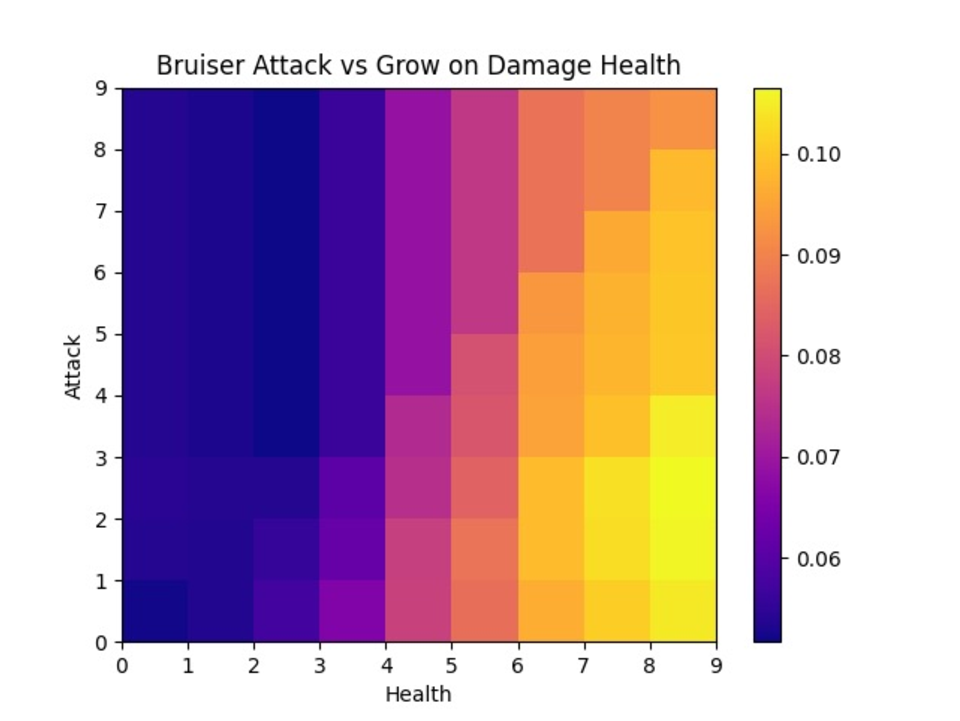
\includegraphics[scale=0.5]{bruiser_vs_grow} 
	\caption{Heatmap showing how changes in the attack of the bruiser card and the health of the grow-on-damage card, while all other card parameters remain fixed, affect the standard deviation metric.}
	\label{fig:bruiser_vs_grow}
\end{figure}

Take, for example, the plot in Figure~\ref{fig:bruiser_vs_grow} of the value of the standard deviation metric given various values for the attack of the bruiser card and the health of the grow-on-damage card. The bruiser card is a vanilla card with a high attack (although variable in this situation) and one health point. The grow-on-damage card has one attack growth per hit. Initially this card has one attack, and in this situation has a variable amount of health. If the grow on damage card is able to consistently become a powerful threat, it can become too strong and a necessity for high-level play, leading to an unbalanced metagame.

In the figure, we can see that configurations in the upper left corner, where the attack of the bruiser is greater than the health of the grow on damage card, tend to be much more favorable than the configurations in the lower right corner, where the opposite is true. This evidence supports the intuitive idea that the bruiser's high attack is a good counter to the grow on damage card because the bruiser card can quickly remove the grow on damage card before it has had enough interactions to grow its damage to a large number. This kind of information can be quite useful to a game designer, who can see very clearly that the inclusion of a high-damage card can improve the metagame dramatically if the grow on damage card is found to be too powerful.

The second plot is a histogram of the lineup win rates after running a tournament amongst all possible lineups. %, the win rates of each lineup are plotted in a histogram.
The resulting distribution can have features that may be informative to %human
game designers. For example, examine the difference between the distributions %shown
in Figures~\ref{fig:special_only_dist_before} and~\ref{fig:special_only_dist_after} from tournaments using two configurations of the same card parameters. 

% TODO: Continue generating more distribution plots, and with other metrics perhaps. And metric discrepancy between logs and pickle file. Investigate length of games.
\begin{figure}[t]
	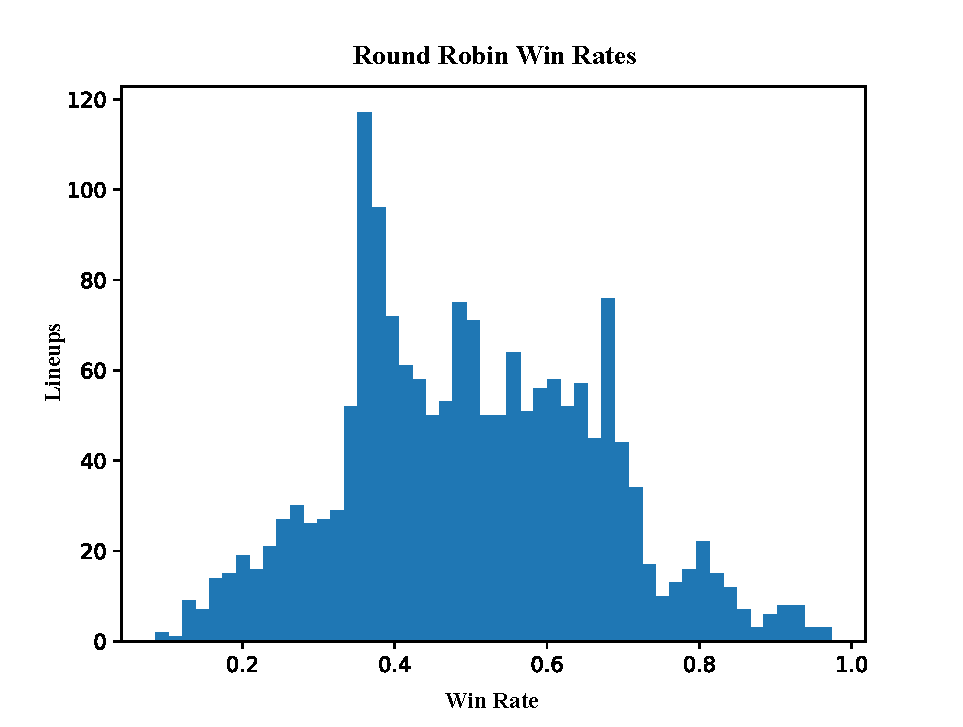
\includegraphics[scale=0.5]{special_only_4_5_8_8_4_8_3_3_3_5}
	\caption{Distribution of win rates before optimization. }
	\label{fig:special_only_dist_before}

	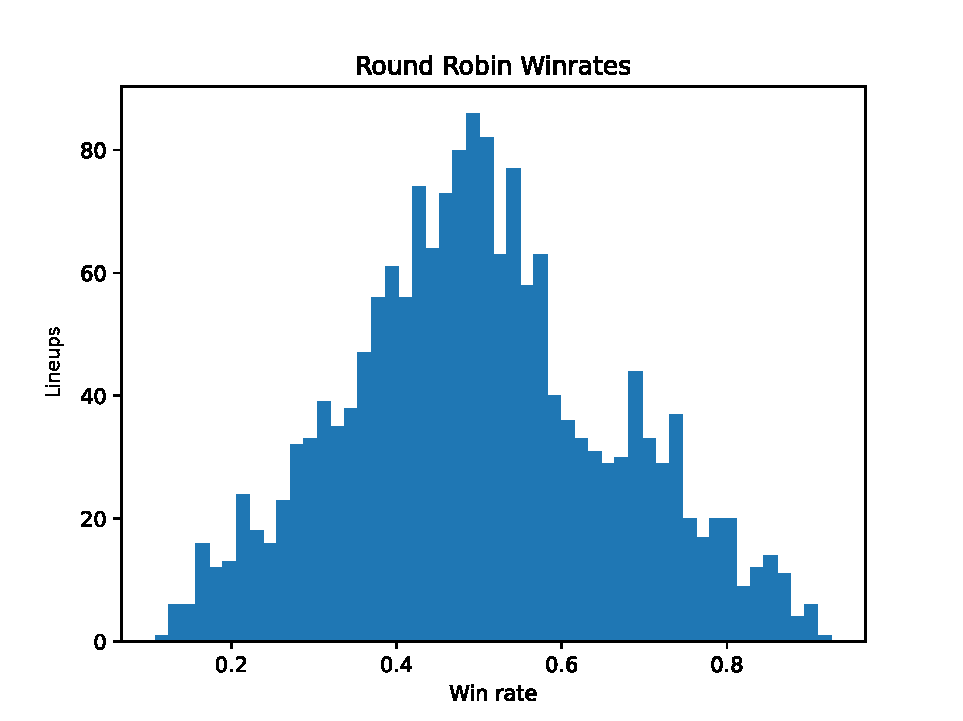
\includegraphics[scale=0.5]{special_only_1_3_4_3_3_1_7_8_5_7}
	\caption{Distribution of win rates after optimization. }
	\label{fig:special_only_dist_after}
\end{figure}

Given playtesting input from actual players and historical data from other successful metagames, game designers can interpret the %understand the what
changes new cards have brought and implement changes to the game or metrics for optimization that will improve the experience of human players.

\subsection{Experiment Design}

% in methods: only describe the phases of experiments in a high level -- 1. build lineups 2. tournaments 3. ... their common pattern
% describe set up, techniques; write about analysis and numbers in results

Our experiments share common phases.

\begin{enumerate}
	\item Build lineups. We generate a set of cards and their associated attack, health points, and special parameters.
	Depending on the experiment, a subset of these parameters may vary between simulations during the optimization process.
	From this set of cards, the lineups are permutations of 3 cards from the set, allowing for duplicates.
	\item Run tournaments. This will be either be a group or a round-robin tournament as described in Section~\ref{sec:tourney}.
	\item Optimize. These tournaments are run within each iteration of our genetic algorithm to produce a metric estimating the best
	possible health of the metagame with respect to configurations of the card parameters. %of the built lineups.
\end{enumerate}

\section{Results} \label{sec:results}
We explore applications of {\sc Ludus} to problems that game designers commonly face.

\subsection{Group Versus Round-Robin Tournament}

% Maybe explain the group tournament in more detail
The first experiment %we ran
investigates the efficacy of our sampling-based approximation in Section~\ref{sec:tourney}. To do this, we compare the win rates %identical lineups in
of a complete round-robin tournament (every combination of lineups played) with the distribution of win rates over a 16-fold tournament of %conducted by
randomly partitioned lineups into groups of various sizes, playing every combination of the lineups within those groups.

\begin{figure}[t]
	\centering
	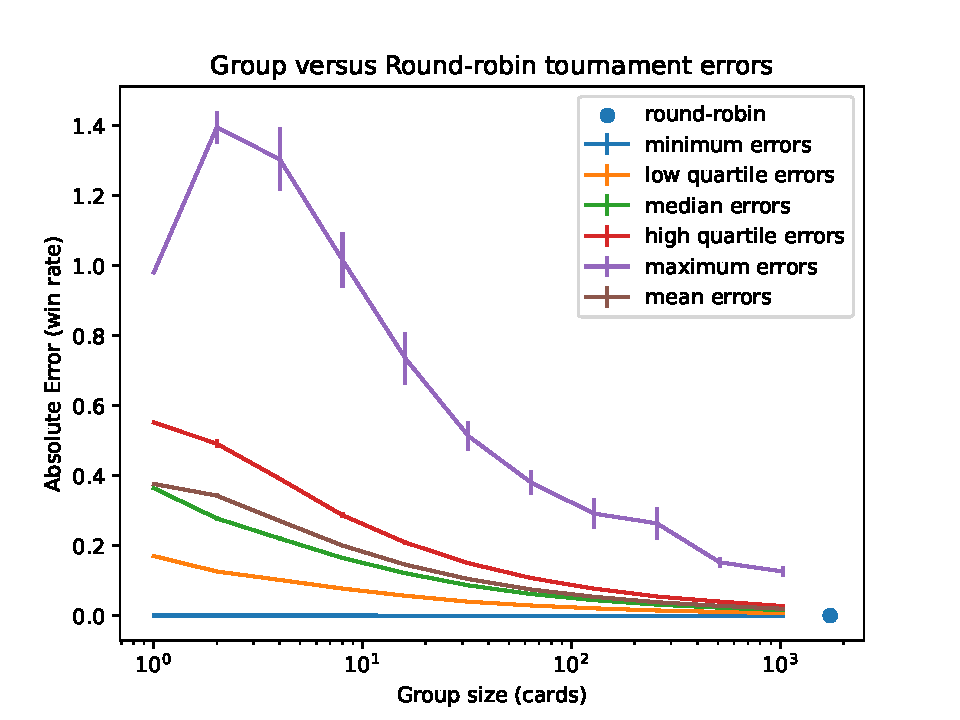
\includegraphics[width=0.88\columnwidth]{group_vs_rr_fig}
	\caption{Absolute value of the difference in win rate between a \textit{group tournament} of varying size and a full round-robin tournament of 1,728 possible lineups. %, along with error bars.
	}
	\label{fig:group_vs_rr}
\end{figure}

%% Table

Figure~\ref{fig:group_vs_rr} compares the win rates of each lineup in the group tournament versus the round-robin tournament, and we can see that at a group size of 256, the mean error becomes negligible (about 0.0382). We use this group size in the other experiments rather than a round-robin of all 1,728 lineups.

% Another table

 \subsection{Optimizing Cards without Special Mechanics}

The next experiment optimizes a set of four `vanilla' cards with no extra mechanics. We expected that the `optimal' solution in terms of the standard deviation metric would have four identical cards because the interchangeable cards should have zero standard deviation in the win rate. Due to the limited number of generations in our genetic algorithm, we recognized that there was no guarantee it would find this solution. From a game design perspective, a less-optimal solution seems more interesting in this case as a game with only a single card is obviously uninteresting. We wanted to see what `almost-optimal' solutions appear for this setup. This observation also illustrates a case where the standard deviation metric fails to fully capture the qualities we wish to optimize in our game.

The results of this experiment illustrate a different failure case of our standard deviation metric that we did not predict. The genetic algorithm quickly found the solution (5/3), (5/4), (8/3), (8/1) where ($a$,$b$) indicates a card with $a$ attack and $b$ health points. This solution had the optimal zero standard deviation---why? Any pairing of these cards will result in both cards killing each other simultaneously. Thus, every game ends after one round of combat phases in a tie, and there is no variance in win rates amongst the lineups. 

 \subsection{Optimizing Only Special Mechanics}

The third experiment optimizes only the special mechanic parameters of twelve cards. We assigned each card an intuitive value for its attack and health, which a game designer might do for initial context. {\sc Ludus} then optimized the parameters for the special mechanics of these partially-designed cards. We were interested to see how it %feasible it is to optimize the game with
optimized under these constraints and how impactful the special mechanics would be for the overall balance. %of the game.
Table~\ref{tab:special_cards} describes the cards used in this experiment. The optimizer improved the win rate standard deviation from 0.0751 to 0.0589. 

\begin{table*}[t]
\centering
\caption{Variable and Fixed Parameters for the \textit{Optimize Special Mechanics} Experiment}
\label{tab:special_cards}
\begin{tabular}{||c c c c c||} 
 \hline
 Card & Attack & Health & Special Parameter (see Section~\ref{sec:ab-game-def}) &  Optimized Special parameter\\ [0.5ex] 
 \hline\hline
 Explode On Death & 2 & 1 & Explosion Damage & 1\\ 
 \hline
 Friendly Vampire & 1 & 3 & Heal Amount & 3 \\
 \hline
 Grow On Damage & 0 & 5 & Attack Growth Per Hit & 4 \\
 \hline
 Heal On Death & 1 & 2 & Explosion Health & 3 \\
 \hline
 Health Donor & 1 & 4 & Heal Donation Percent & 3 \\
 \hline
 Ignore First Damage & 2 & 1 & Armor Points & 1 \\
 \hline
 Morph Attack & 0 & 3 & Morphing Enemies & N/A \\
 \hline
 Pain Splitter & 2 & 2 & Damage Split Percent & 7 \\
 \hline
 Rampage & 0 & 4 & Middle Age & 8 \\
 \hline
 Survivalist & 2 & 2 & Survivalist & N/A \\
 \hline
 Threshold & 2 & 2 & Target Age & 5 \\
 \hline
 Time Bomb & 1 & 8 & Detonation Time & 7 \\ 
 \hline
\end{tabular}
\end{table*}

\subsection{Optimizing All Parameters} \label{sec:first_set}

After fixing the attack and health to focus solely on the special mechanics, the next experiment tunes the attack, health, and special mechanics all at once. To reduce the huge dimensionality of this experiment, we selected only five of the twelve cards to optimize. They are listed in Table~\ref{tab:first_set}.

% First Set
\begin{table*}[t]
\centering
\caption{List of Cards in the First Set and Their Optimized Solution}
\label{tab:first_set}
\begin{tabular}{||c c c c||} 
 \hline
 Card & Optimized Attack & Optimized Health & Optimized Special Mechanic (see Section~\ref{sec:ab-game-def})\\ [0.5ex]
 \hline\hline
 Survivalist & 9 & 1 & N/A \\
 \hline
 Morph Attack & 5 & 5 & N/A \\
 \hline
 Ignore First Damage & 6 & 8 & 1 \\
 \hline
 Explode On Death & 4 & 1 & 3 \\ 
 \hline
 Vanilla & 7 & 2 & N/A \\
 \hline
\end{tabular}
%\end{table*}

% Second Set
%\begin{table*}[t]
%\centering
\caption{List of Cards in the Second Set and Their Optimized Solution}
\label{tab:second_set}
\begin{tabular}{||c c c c||} 
 \hline
 Card & Optimized Attack & Optimized Health & Optimized Special Mechanic (see Section~\ref{sec:ab-game-def})\\ [0.5ex]
 \hline\hline
 Friendly Vampire & 7 & 7 & 8 \\
 \hline
 Grow On Damage & 2 & 6 & 9 \\
 \hline
 Heal On Death & 3 & 9 & 1 \\
 \hline
 Rampage & 6 & 7 & 5 \\ 
 \hline
 Vanilla & 7 & 6 & N/A \\
 \hline
\end{tabular}
\end{table*}


The optimizer improved the win rate standard deviation from 0.0704 to 0.0584. This minimum is approximately the same as the one achieved in the previous experiment, modifying only the values of the special mechanics. One important observation we made is that the optimizer was still making good progress in the final generations of both our experiments. This indicates that these might not be minima, %are not global, but that with
and compute time for additional generations could continue to improve the card designs.


\subsection{Optimizing After a Set Rotation}

Another common scenario designers of deck-building games encounter is releasing a new set %or batch
of cards that maintain the compatibility, fairness, and competitiveness with the previously released cards. %These expansions add new content to the game to keep it fresh.
To apply {\sc Ludus} to this problem, we took the set of five cards from Section~\ref{sec:first_set} with their optimized solution as %This represents
the first set of cards released. Next, we selected five additional cards, described in table Table~\ref{tab:second_set}, and optimized them alongside %, while keeping the values from
the first set fixed at the solution found previously---this is ten cards with variable parameters for only the second set of cards. 

% Compare this to the solution found by treating all 10 cards as one set

The optimizer improved the win rate standard deviation from 0.0591 to 0.0541. This is a comparatively smaller improvement than the previous experiments, %however,
but the initial state was already in much better condition than any of the previous experiments. This is interesting because it could indicate that adding new cards to an already well-balanced set may not disturb the balance as much as one might expect. 

\section{Discussion} \label{sec:discussion}
We can see that the {\sc Ludus} framework yielded some very useful results from a game design perspective. Given a small, yet representative, set of cards, our methods were able to find more balanced configurations for cards that should create a far more enjoyable auto battler game to play.

We also implemented an approximation method that considerably reduces the computation time necessary to evaluate configurations during optimization, especially for large card sets. This method randomly breaks the tournament into smaller groups that only compete within themselves. Our empirical results indicate that under most circumstances, the approximations are close enough to the %result of the
complete tournament to produce satisfactory optimization results. 

We applied the {\sc Ludus} framework to some standard problems game designers face and found promising results. Notably, the algorithm successfully optimized cards under various constraints from partially-designed cards to expansions of %a second set of cards after fixing a first, previously optimized, set.
previously optimized card sets.

Beyond the immediate results of this paper, we contributed an auto battler game and its associated tools. %to the literature.
Given the recent nature of this genre, we believe this is an important contribution that will aid future research in the area.

\section{Future Work} \label{sec:futurework}
The genre of auto battlers is very young, and our research only explores a narrow slice of questions in this new area. We discuss problems that extend our current work.

\subsection{Other Auto Battler Features}

% draft phase of auto battlers

Unlike our game, some auto battlers have
players iteratively build their lineup between battles by purchasing
cards from an array of options. While our experiments were concerned with fixed lineups of size 3, 
{\sc Ludus}'s ability to quantify, qualify, and optimize balance for other deck-building rules %with more or fewer cards
remains to be assessed. We previously only considered
the case where any card may be replaced with any other card to create a new lineup. However, 
the purchasing value of cards is another dimension of their design; %may be different and
future work should consider comparing lineups
that players can build after the same number of battles and purchasing phases.

% cards with multiple mechanics

In many auto battlers, cards have multiple special mechanics that each have variable parameters.
Our work only considers cards with a single mechanic, but this should be extended to optimize design for such cards.

% non-determinism/random effects? is this in other games besides heartstone battlegrouds?

\subsection{Simulation Data}

All metrics we present are based off of the average win rates of lineups collected from the simulator. 
This does not take into account individual lineup-versus-lineup win rates, which are always 0 or 1 since
our auto battler game is deterministic. One could represent these relations via a
\textit{domination graph} with lineups
as nodes and a directed edge to the lineup that wins the head-to-head matchup \cite{gkmmmf_eaai21},
game matrices with each lineup as a strategy, and more.
%The size of these data structures
%scale quadratically with the number of lineups just like the round-robin tournament, which means more sampling-based approximation would be necessary in practice.
Further investigation is required to determine whether perturbations of card parameters causing a degradation
in metagame health correspond to any changes in these representations.  There are also game design factors to consider besides win rates, such as game durations and intensity levels.
\if{false}
construct a \textit{domination graph} with lineups
as nodes and a directed edge to the lineup that wins the head-to-head matchup. The size of the domination
graph problematically scales with the square of the number of lineups just like the round-robin tournament,
so another sampling method would be necessary in practice. Further investigation is required to determine if perturbation of card parameters causing a degradation
in metagame health corresponds to any phase transition in a domination graph.
\fi

% We don't consider lineup vs lineup win rates, only average win rates

% mention our original pareto idea?

\subsection{Alternative Optimization Methods}

Our choice of a genetic algorithm for optimization is somewhat arbitrary. Genetic algorithms can conveniently 
handle the familiar integer values of card parameters, unlike other optimization methods. Gradient- and Hessian-based
methods in particular are difficult to apply to this problem due to its discrete nature and our simulator not being
differentiable. Had they been applicable, they would have solved an unmet need of %qualifying
validating the stability of optimization
results. %with respect to the variable parameters.

\subsection{Human Playtesting}

Human playtesting is still required to determine the health of the metagame as we have not verified to what extent our metrics
correspond to what humans deem as a healthy metagame. Designers
with a historically healthy metagame can use those parameters to generate reference win rate distributions 
over lineups and cards using our {\sc Ludus} framework. These distributions can then shape 
new metrics and imply their ideal values for parity. Human playtesting feedback could also motivate other metrics based on the gameplay experience,
such as the number of turns. %in each match.
While this work is an example of how designers can readily apply the {\sc Ludus} framework,
researching human playtesting-validated results marks an important avenue of 
future work.

\section{Acknowledgments}
The authors would like the thank the anonymous reviewers for their helpful feedback, Nathan Ringo for providing computational resources to run the experiments, and everyone at SIFT for their support.

\bibliography{eaai22_bgmmwlf}
\end{document}
